\chapter{Objectives}
\label{chap:2_objectives}
Once we have presented the introductory context of this project, we will describe its objectives, along to the followed methodology to achieve all of them.\\

The final objective is to enrich the JdeRobot platform on its Computer Vision aspect, upgrading an existing component and creating two consecutive new ones. Keeping this in mind, we will be able to generate a behavioral focused, as a specific application, on tracking and actively following a person, making use of a robot. This internal process of transformation of a stimulus into a reactive movement will be accomplished using \textit{Convolutional Neural Networks}.\\


\section{Main objectives}

		\subsection{Classification}
			Our first objective (and the first task to tackle) will be to upgrade the support of the digit classification tool already existent in JdeRobot, \texttt{DigitClassifier} (\autoref{sec:3_digitclassifier_jderobot}). This will allow us to augment the scope of this component, due to the support for the new framework, TensorFlow (\autoref{sec:3_tensorflow}). This is a good starting point to achieve some initial skills building and training Convolutional Neural Networks on TensorFlow (it will be the main framework used all along the project).\\
		
		
		\subsection{Detection}
			As it will be described on the suitable chapter, we will build a component (\texttt{ObjectDetector}) which deploys \textit{a generic object detection algorithm} on an incoming video stream. This component will be ready to work in \emph{real time}. It will also be compatible with new network models (e.g. a new detection model trained by us), which will be loaded transparently at runtime.\\
			
			As it can be inferred, it will not provide a response \textit{per se}. Its visible output will be to draw \emph{bounding boxes} surrounding each detected object, indicating as well the class where that particular object belongs (person, airplane, dog, etc.), and its score (confidence in \%).\\
		
		\subsection{Tracking and following}
			As an example of the plethora of possible applications of the previous described objective/milestone (object detection on an image), we want to implement a ``person following" behavioral. Our main objective here is to \textit{identify and track} the person to follow, which will semantically be called \emph{mom}. The component that comprehends the previous detection behavioral and this new one will be named \texttt{FollowPerson}. The great advantage here is the strength a CNN can achieve under variable light conditions. That makes this technique perfectly suitable to command physical actuators on a robot.\\
			
			We will make use of the detected people (with the technique followed on the previously described node and constraining the result to only retain people detection), and look for the face of each one of them. Later, we will make use of another neural network technique, called a \emph{siamese network} (it will be properly explained later) to identify them. It will allow us to find \emph{mom}, in case it is being seen by the camera, and command a proper response to the robot with the objective of following \emph{mom}.\\
			
			\vspace{1in}

As we have said before, these two last nodes/components are successive. Thus, they will share an important part of the global objectives.\\

We will start breaking down the common objectives between both applications, into three functional blocks:

\begin{itemize}
	\item \textit{Design:} both milestones have been preceded by a first \textit{documentation} phase. While the theoretical base was learned and achieved, some papers and examples were investigated. We will go some deeper in each section.
	
	Later, a more specific design phase will be to specify the structure of the nodes.
	From now on, we will have to perform several tasks simultaneously:
	\begin{itemize}
		\item Grabbing the incoming image(s) from the sensor(s).
		\item Processing the image(s).
		\item Properly update the GUI (\textit{Graphical User Interface}) with the image(s) and the outputs of the processing.
		\item \textit{Only on the following node:} send the computed response order to the actuators.
	\end{itemize}
	%
	These tasks should follow an \emph{asynchronous schema} every time, to avoid blocks between tasks, and taking advantage of some shared memory to exchange inputs/outputs. Besides, this allows us to have a custom iteration period for each task: we shouldn't have to wait until the neural network finishes feed-forwarding the image to refresh the \emph{GUI}. On a high level structure, it could follow the schema on the \autoref{fig:2_tasks}.
	
	\begin{figure}[h]
		\centering
		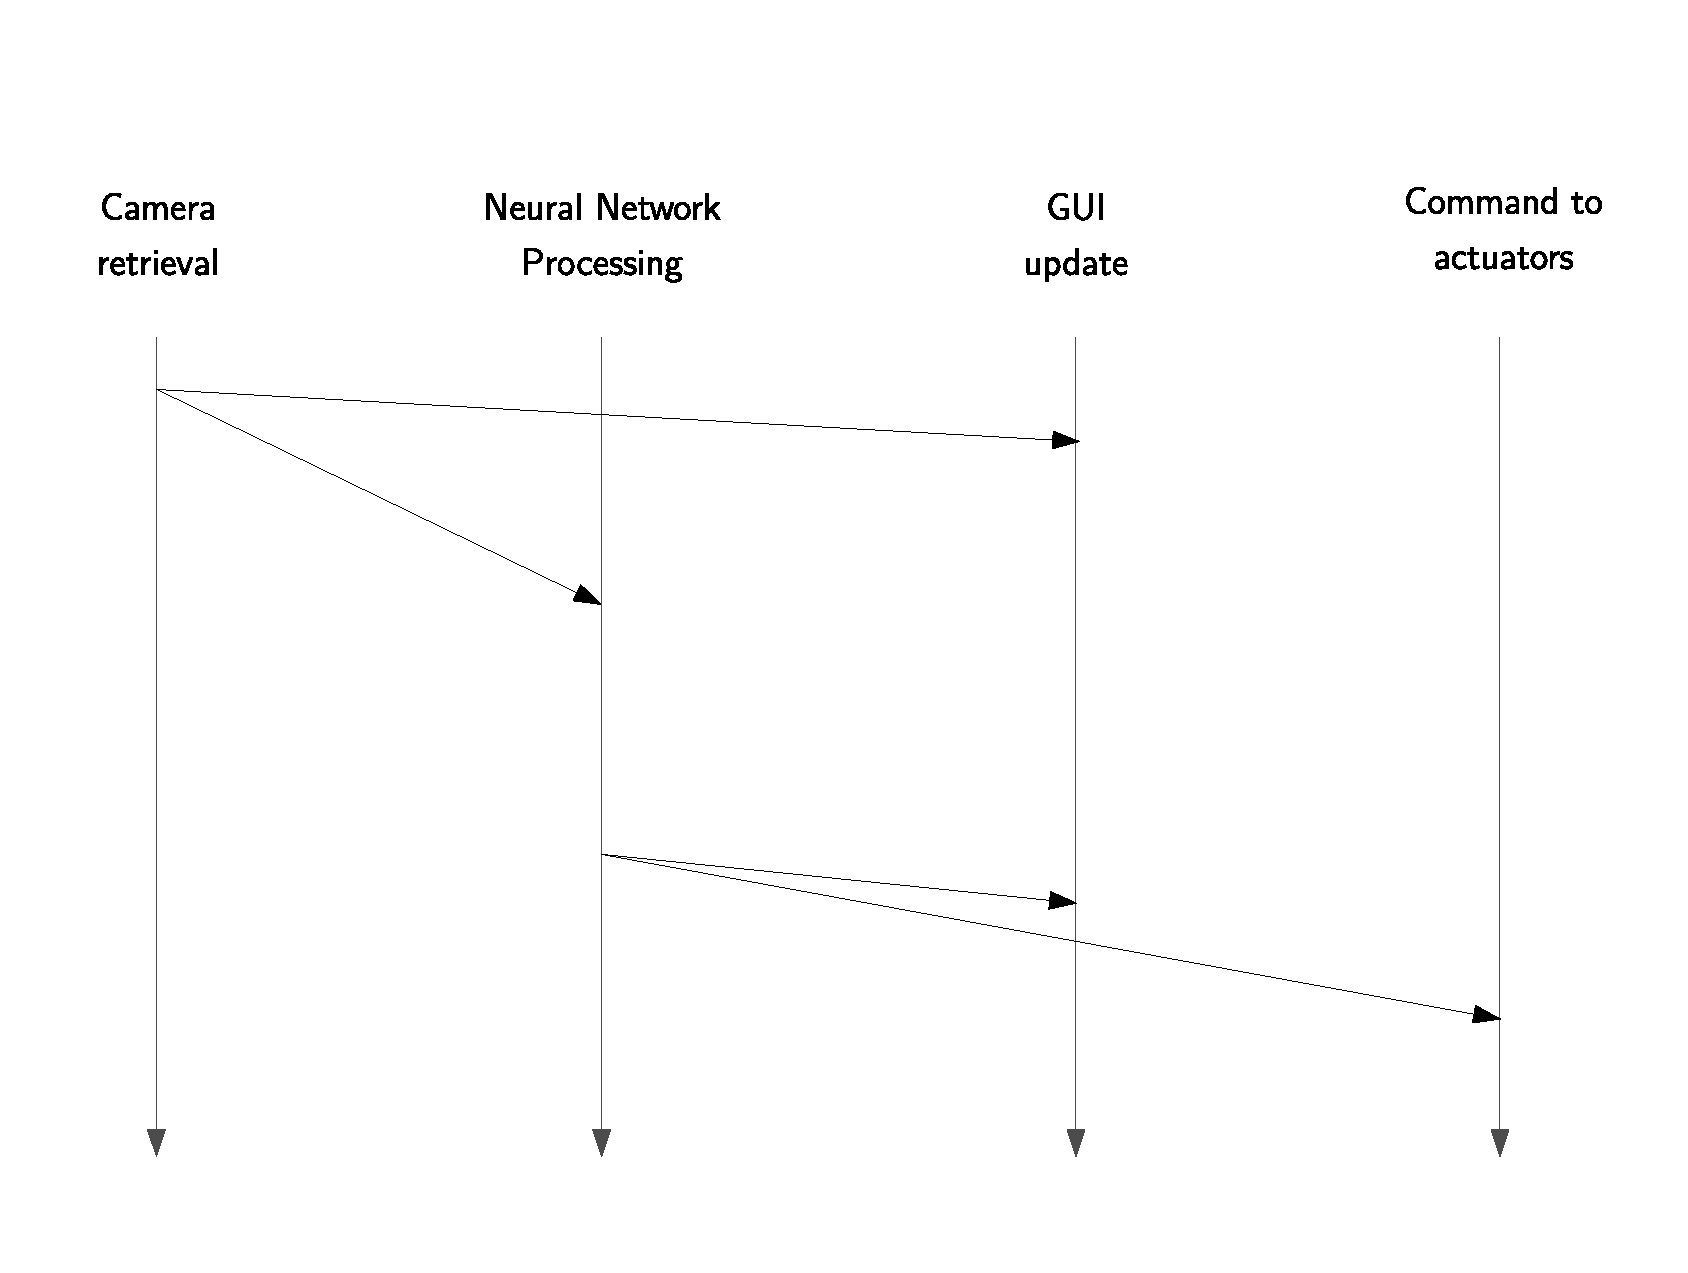
\includegraphics[width=4in]{images/tasks_threads}
		\caption{Parallel tasks to perform, and data exchange between them.}
		\label{fig:2_tasks}
	\end{figure}
	
	\item \textit{Implementation:} the next and most time consuming objective is to \textit{develop both components}. The advantage is, once again, that both components are successive. This makes code reutilization a very interesting move, as we will only need to perform a language-friendly additions (on a simple way, thanks to \textit{Object Oriented Programming})) to the \texttt{Object Detector} code to implement the \texttt{Follow Person} features (depth images support, computing and commanding movements to the motors, among others). Details will be described on the appropriate section.
	
	\item \textit{Experimentation\footnote{\textit{"In theory, theory and practice are the same. In practice, they are not."}, Y. Berra}:} these nodes have a very strong tunability component (from neural network parameters to movement factors in the commands for the motors, stopping over describing all the desired behavior that the following algorithm has to adopt in several situations that it has to be capable of handling).
	
\end{itemize}

Finally, we will briefly highlight the \textit{personal} objectives we have pursued on this project. As this has been developed along a whole year, and on a relatively abstract field as \emph{deep learning} is, a level of rigour has been necessary to accomplish satisfactory results. This provides a novice investigator the opportunity to learn about the phases and development process on a much more professional way than a homework task. \\

In addition, this project has allowed an interested person in \emph{deep learning} to learn about a cornucopia of concepts and experience. Later, when it was decided to evolve towards creating a reactive behavioral, it was motivating to make the most of a possible synergy between two different fields of knowledge, as \emph{deep learning} and \emph{robotics} are. It has to be remarked that the implementation of the development has always been possible, so it has been easy where there was more work to do in every moment.

\section{Methodology}
The development of this project, as it has been described, has been subdivided into smaller tasks, or \emph{prototypes}, which could be addressed as individual tasks to achieve. The way to tackle them has been a \textit{spiral methodology} \cite{boehm-spiral}.\\

\begin{figure}[h]
	\centering
	\includegraphics[width=4in]{images/spiral}
	\caption{Spiral Development Model.}
	\label{fig:2_spiral}
\end{figure}

This consists on a software development work procedure that, on a general outline, is very similar to a conch. It describes a 4 phases methodology \cite{spiral-steps}, explained right below:

\begin{enumerate}
	\item \textit{Planning:} establishing the objectives to tackle on the incoming work iteration.

	\item \textit{Risk Analysis:} Later, we evaluate the possible risks and dangers we can find developing the specific program(s). For each found risk, we will try to find a solution to solve or, at least, mitigate it beforehand.

	\item \textit{Development \& testing:} This phase is purely focused on writing the planned piece of software, following the guidelines obtained on the previous steps. In addition, corresponding tests should be performed to check that the work will accomplish the asked functionality.
	\item \textit{Evaluation:} Lastly, when the development phase has been finished, an evaluation has to be performed on the results. This will be the key to know if it is compliant with the initial requirements and if, hence, its development has been successful.
\end{enumerate}

As this was the general procedure followed for each iteration of the developed software, the completion of the evaluation phase immediately led to another planning phase, already belonging to the next iteration. As this is a cyclic process, we can perform as many iterations as desired, slightly increasing the scope of the project on each new one.\\

The workflow present on this project has been supported by weekly meetings, scheduled in order to get up-to-date with the last established objectives and tasks, and set up the work until the next one. This has allowed to keep a constant feedback with the tutor and hold the followed path onto the desired direction.\\

Additionally, a MediaWiki page\footnote{\url{https://jderobot.org/Naxvm-tfg}} has been mantained on the JdeRobot website, reflecting every effort and achievement in order to have a good temporal reference of the work done, and a timeline of accomplishments, and including demonstration videos for each successful iteration result.\\

The code for all the project has been handled on the GitHub repository\footnote{\url{https://github.com/RoboticsURJC-Students/2017-tfg-nacho\_condes}} created for this purpose. However, as the resulting nodes were officially incorporated to the JdeRobot environment, they were migrated to their own repositories. This will be further described on the section dedicated to each component/iteration.\\


\section{Requirements}

For every covered topic, the developed solution must be compliant with the requirements formulated below:

\begin{itemize}
	\item 
\end{itemize}
